\documentclass{article}
\usepackage{float}
\usepackage{graphicx}

\graphicspath{ {../figures/} }
\parindent=0in

\title{MuckRock News FOIA Request Analysis}
\author{Karson Kimbrel}

\begin{document}
	\pagestyle{empty}
	
	\maketitle
	
	\section{Abstract}
	In this paper we discuss the 
	
	\section{Introduction}
	
	
	\section{Goals}
	
	
	\subsection{Major Goals}
		\begin{itemize}
			\item Determine the most successful time(s) of year
			\item Predict acceptance/rejection
			\item Determine the most open agencies
			\item Determine the most open juristictions
		\end{itemize}
	
	\subsection{Minor Goals}
		\begin{itemize}
			\item Lexigraphical analysis on accepted FOIA requests vs rejected requests
		\end{itemize}
	
	\section{Definitions}
		Fully Successful FOIA Request - A FOIA request that was granted in full.\\
		Partially Successful FOIA Request - A FOIA request that was granted or denied in part.\\
		Failed Request - A FOIA request that was ignored, denied, or granted but did not have any records that responded to the request.\\
	
	\section{Method}
	
	
	\section{Results}
	
		\begin{figure}[H]
			\centering
			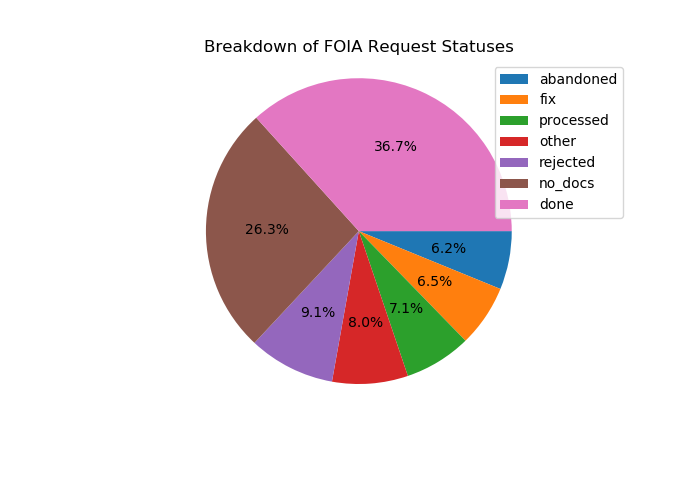
\includegraphics[width=0.75\textwidth]{statuses}
			\caption{Breakdown of all FOIA requests}
			\label{fig:statuses}
		\end{figure}
	
		\begin{figure}[H]
			\centering
			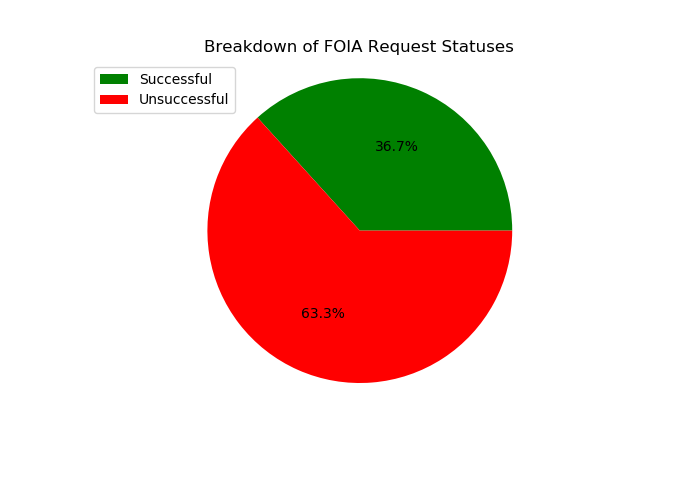
\includegraphics[width=0.75\textwidth]{statuses_simple}
			\caption{Breakdown of all FOIA requests (sorted into successful and unsuccessful requests)}
			\label{fig:statuses_simple}
		\end{figure}
	
		\begin{figure}[H]
			\centering
			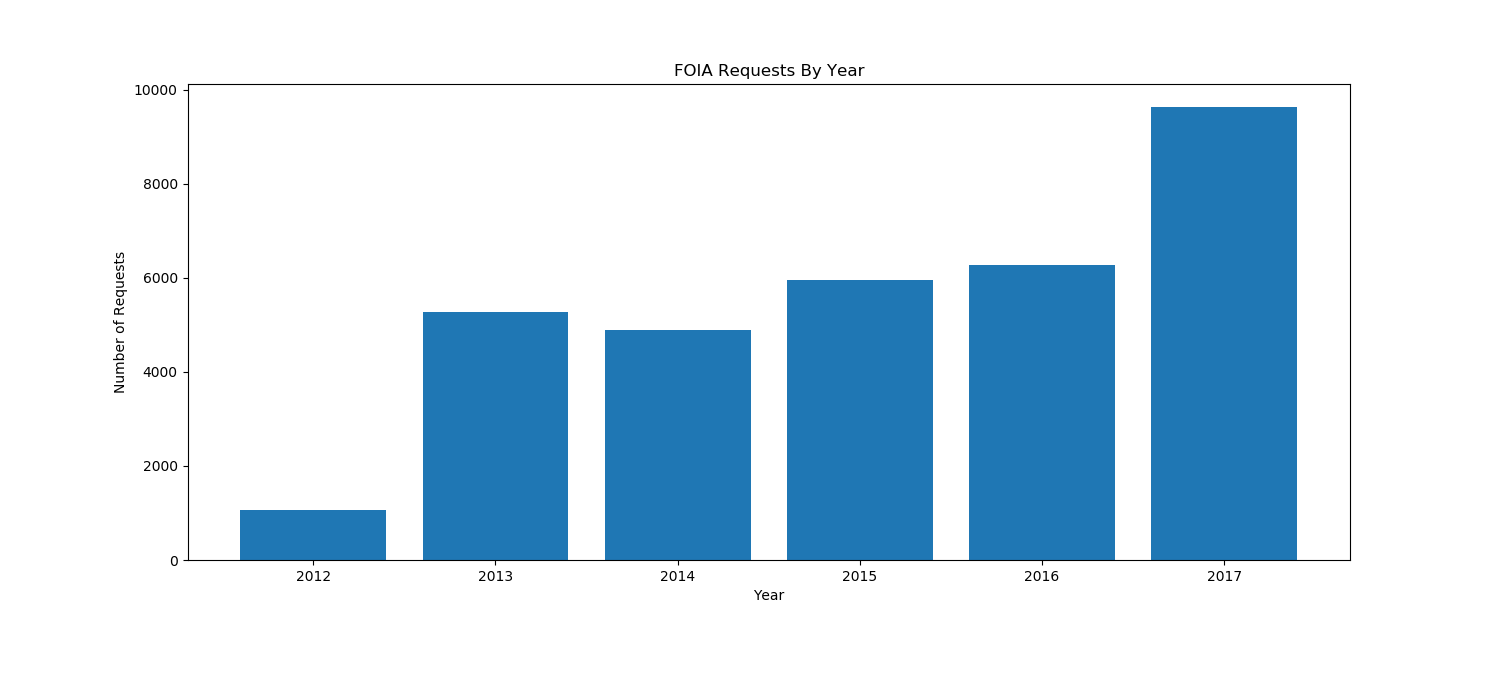
\includegraphics[width=1\textwidth]{yearly_total}
			\caption{The total number of requests by year}
			\label{fig:yearly_total}
		\end{figure}
	
		\begin{figure}[H]
			\centering
			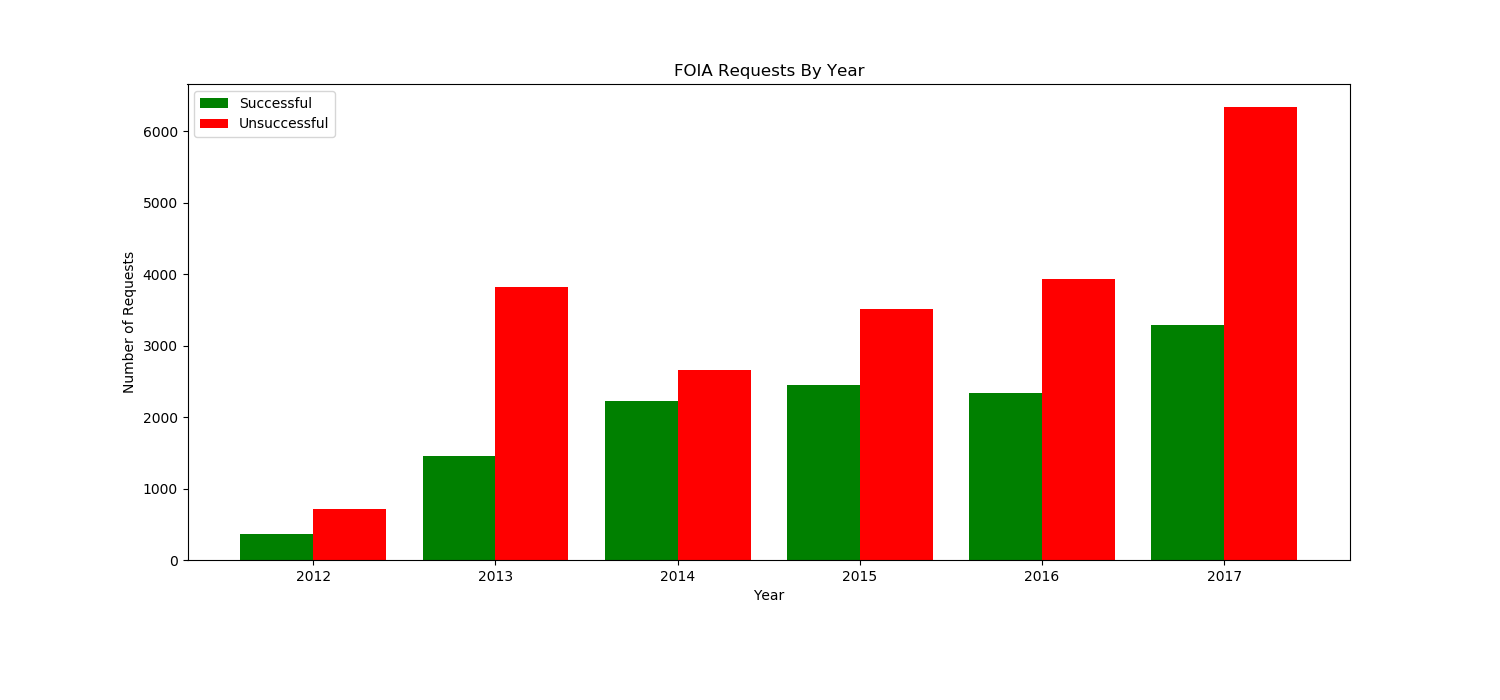
\includegraphics[width=1\textwidth]{yearly_breakdown}
			\caption{The total number of requests by year broken into successful and unsuccessful categories}
			\label{fig:yearly_breakdown}
		\end{figure}
	
		\begin{figure}[H]
			\centering
			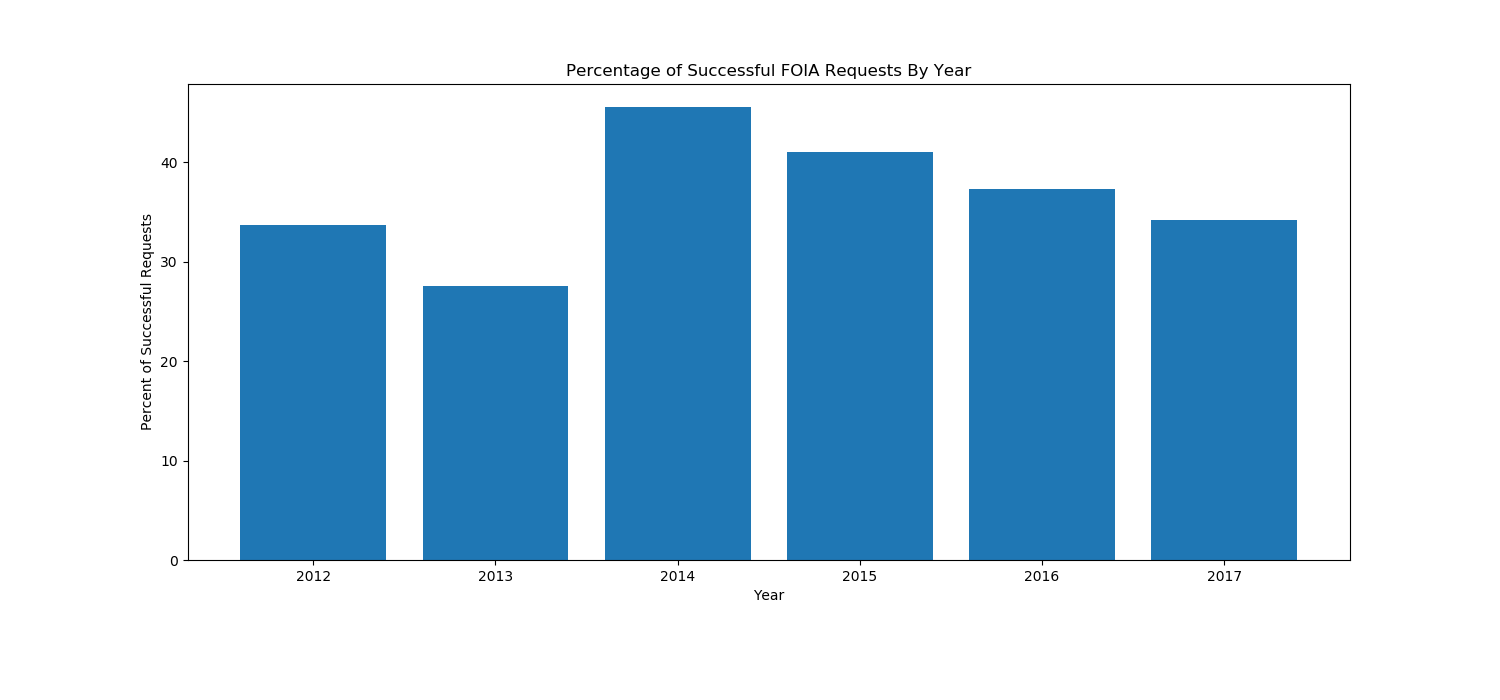
\includegraphics[width=1\textwidth]{yearly_percent_successful}
			\caption{The percentage of successful FOIA requests by year}
			\label{fig:yearly_percent_successful}
		\end{figure}
	
		\begin{figure}[H]
			\centering
			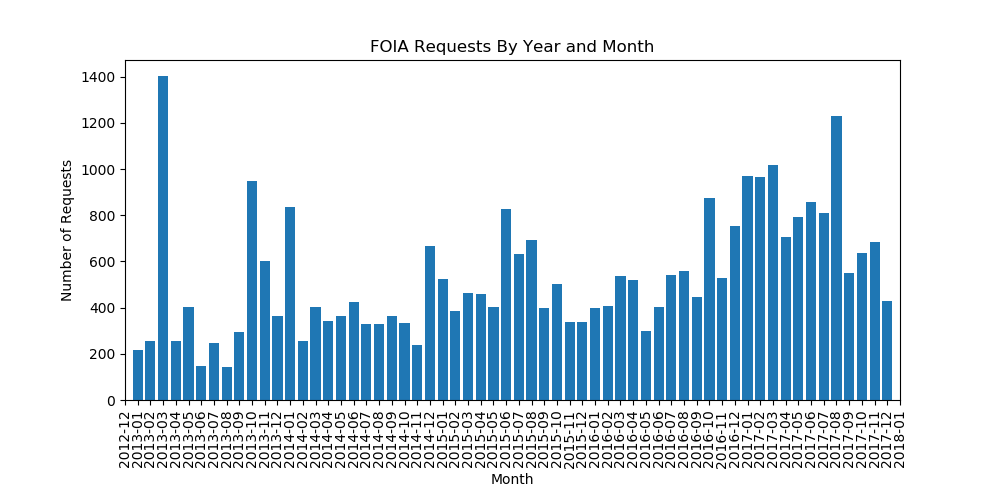
\includegraphics[width=1\textwidth]{monthly_total}
			\caption{The total number of requests by year and month}
			\label{fig:monthly_total}
		\end{figure}
	
		\begin{figure}[H]
			\centering
			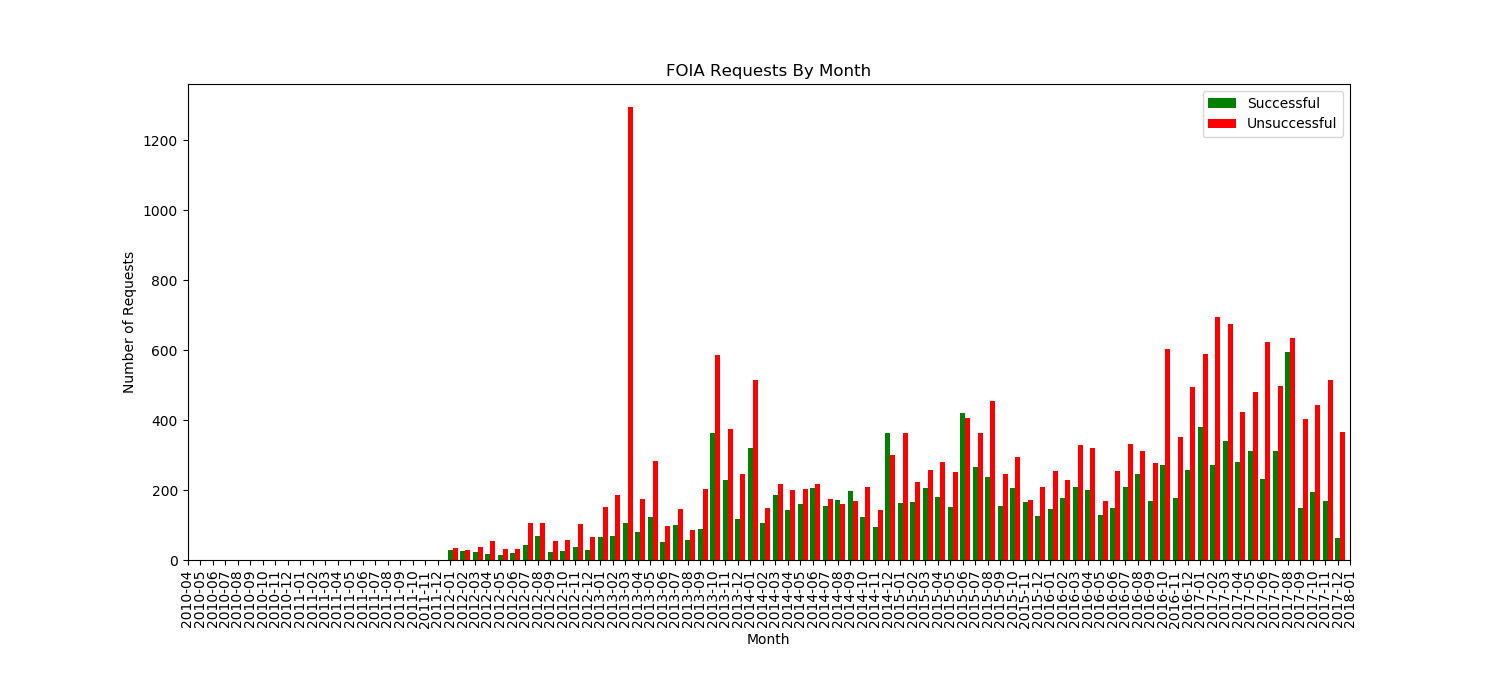
\includegraphics[width=1\textwidth]{monthly_breakdown}
			\caption{The total number of requests by year and month broken into successful and unsuccessful categories}
			\label{fig:monthly_breakdown}
		\end{figure}
	
		\begin{figure}[H]
			\centering
			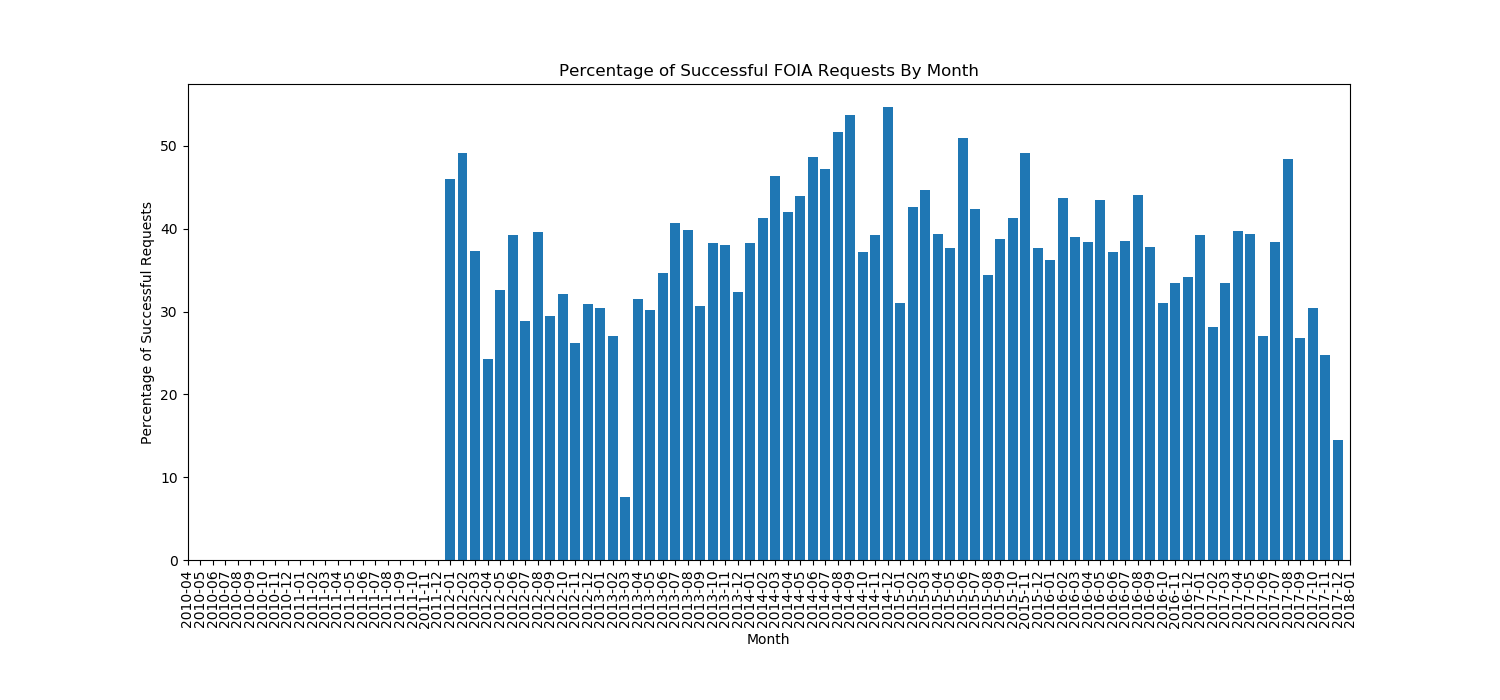
\includegraphics[width=1\textwidth]{monthly_percent_successful}
			\caption{The percentage of successful FOIA requests by year and month}
			\label{fig:monthly_percent_successful}
		\end{figure}
	
	\section{Discussion}
	
	
	\section{Conclusion}
	
	
	\section{References}
	
	
	\section{Acknowledgements}

\end{document}